\selectlanguage{italian}%

\section{Soluzione}


\subsection{Schematici}

\subsubsection{Display a 7 segmenti}

\label{subsec:display}

L'approccio di design adottato � rappresentato dallo schematico dell'architettura
in figura \ref{fig:display}.

\begin{figure}[H]
	\centering
	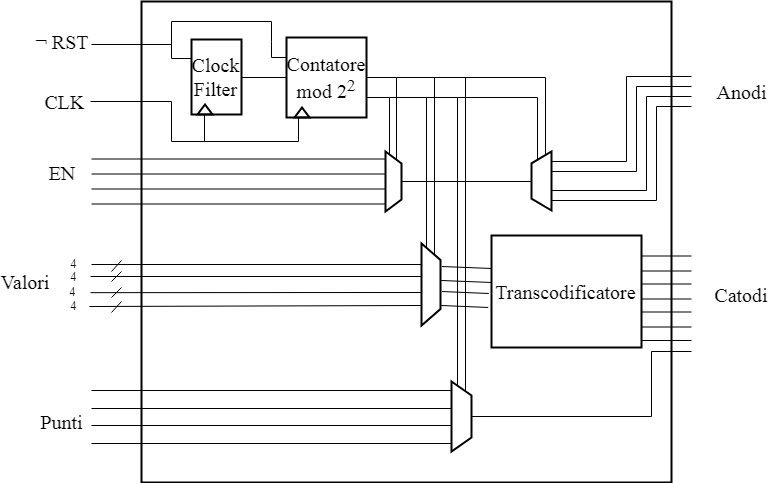
\includegraphics[scale=0.7]{esercizio04/images/Display.png}
	\caption{Architettura del display a sette segmenti}
	\label{fig:display}
\end{figure}

Gli input sono rappresentati da: un segnale di clock, uno di reset
in logica 0 attiva, le abilitazioni per le quattro cifre del display,
i valori che le stesse cifre devono assumere e l'eventuale posizione
dei punti da accendere. Gli output sono costituiti dai segnali degli
anodi comuni ai sette segmenti, uno per ciascuna cifra, e dai segnali
dei catodi, sette dei quali in riferimento ai segmenti della cifra
in questione, l'ultimo relativo al punto ad essa associato.\\
Il segnale di clock � filtrato da un clock filter, che restituisce
un segnale di hit a frequenza minore. Il clock permette, inoltre,
il conteggio al contatore modulo 4, abilitato dal segnale di hit del
clock filter. Il reset, se negato, consente il ripristino del clock
filter e del contatore. L'uscita del contatore consente di selezionare
una cifra del display ad ogni conteggio. Infatti, avendo le quattro
cifre i catodi dei segmenti in comune, per mostrare un valore differente
su ciascuna di esse � necessario un refresh del valore con una frequenza
sufficientemente elevata.\\
I segnali di abilitazione permettono di decidere quali cifre del display
utilizzare. Essi, in ingresso ad un multiplexer 4x1, sono selezionati
dal contatore per considerare in ogni istante l'abilitazione legata
alla cifra corrente. L'abilitazione cos� individuata identifica l'anodo
relativo attraverso un demultiplexer 1x4, sempre tramite la selezione
del contatore. Ad ogni conteggio, la cifra selezionata avr� anodo
basso o alto, a seconda dei valori di abilitazione passati in ingresso.\\
I 16 bit di ingresso dei valori rappresentano i quattro nibble relativi
alle quattro cifre del display. Una struttura di multiplexing seleziona,
in riferimento ai valori di conteggio, il nibble relativo alla cifra
corrente. I 4 bit del nibble entrano in un transcodificatore per la
corretta accensione dei sette segmenti della cifra.\\
L'ottavo catodo della cifra � costituito dal punto ad essa associato.
I quattro segnali di ingresso dei punti, infatti, decretano se il
punto, associato alla cifra selezionata, debba essere acceso, o meno.
Un multiplexer 4x1 seleziona, grazie al conteggio, il valore corretto
da assegnare al punto della cifra corrente.\\
L'implementazione dell'architettura � stata realizzata mediante la
rappresentazione RT Level di figura \ref{fig:impl}.

\begin{figure}[H]
	\centering
	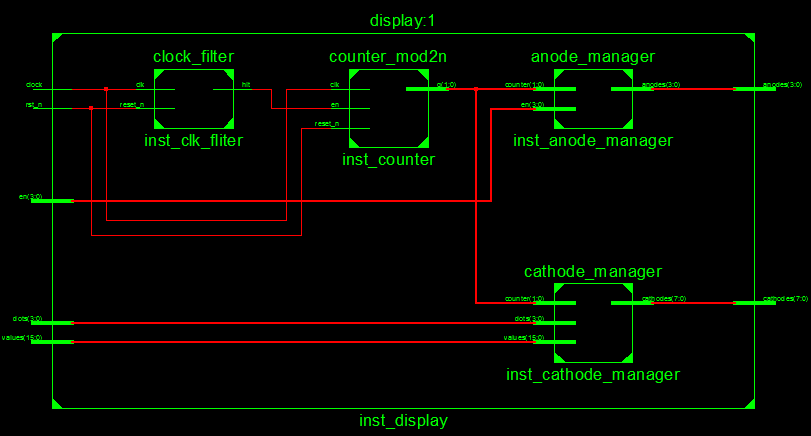
\includegraphics[scale=0.8]{esercizio04/images/Implementazione.png}
	\caption{Display RTL Schematic}
	\label{fig:impl}
\end{figure}

\subsubsection{Struttura di multiplexing 16x4}

\label{subsec:mux16x4}

Esplodiamo l'architettura che consente la selezione del nibble relativo
alla cifra corrente del conteggio. Essa � realizzata mediante 4 multiplexer
4x1, ognuno dei quali riceve in ingresso un bit di pari peso dei nibble
associati alle diverse cifre. L'ingresso di selezione � costituito
dall'uscita del contatore.

\begin{figure}[H]
	\centering
	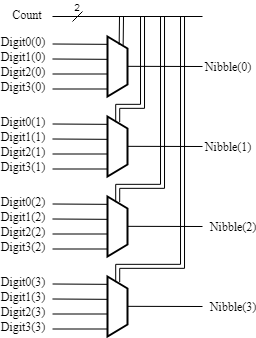
\includegraphics[scale=0.9]{esercizio04/images/Mux16x4.png}
	\caption{Architettura di multiplexing 16x4}
	\label{fig:mux16x4}
\end{figure}

\subsection{Codice}


\subsubsection{Clock Filter}

Il clock filter riceve in ingresso un segnale di reset in logica 0
attiva per ritornare ad uno stato neutro in modo asincrono all'elaborazione
del conteggio. Esso funge da divisore di frequenza, restituendo il
segnale hit con una frequenza sottomultipla di quella del clock in
ingresso. Il rapporto tra le due frequenze rappresenta il numero di
conteggi da effettuare dopo il quale il filtro deve alzare hit (nemero
di colpi di clock in un periodo di hit). Non si � potuto sfruttare
un contatore modulo $2^{N}$ perch� non � detto che il conteggio sia
potenza di 2.

\lstinputlisting [language=VHDL,caption={Definizione del componente Clock Filter}] {esercizio04/codice/clock_filter.vhd}

\subsubsection{Anode Manager}

Il gestore degli anodi utilizza una rete mux-demux per abilitare ad
ogni conteggio l'anodo corretto. L'uscita del contatore rappresenta
l'ingresso di selezione sia per il multiplexer, che per il demultiplexer.
Gli ingressi di abilitazione entrano in un mux 4x1. L'uscita del multiplexer
� posta in ingresso al demultiplexer. Lo stesso segnale di selezione
garantisce che l'abilitazione sar� portata fino all'anodo a cui essa
fa riferimento.

\lstinputlisting [language=VHDL,caption={Definizione del componente Anode Manager}] {esercizio04/codice/anode_manager.vhd}

\subsubsection{Cathode Manager}

Il gestore dei catodi riceve in ingresso il conteggio, i valori che
i catodi dei sette segmenti devono assumere e quelli del catodo dei
punti. L'uscita � costituita dagli 8 segnali dei catodi. Il componente
sfrutta la struttura di multiplexing descritta in \ref{subsec:mux16x4}.
Per fare ci� riordina i valori di ingresso nel modo richiesto dalla
batteria di mux 4x1. Il nibble cos� ottenuto entra nel transcodificatore,
realizzato col componente cathode encoder, dal quale si ottengono
i segnali dei catodi dei sette segmenti. Il segnale dell'ultimo catodo
� ricavato dal multiplexing dei valori dei punti in ingresso: un mux
4x1 determina quale valore porre in uscita sul catodo.

\lstinputlisting [language=VHDL,caption={Definizione del componente Cathode Manager}] {esercizio04/codice/cathode_manager.vhd}

\subsubsection{Cathode\_encoder}

Questo componente effettua la funzione di transcodifica di un nibble
nelle funzioni booleane dei sette segmenti. Esso, dunque, riceve in
input un nibble e restituisce il valore assunto dai catodi dei sette
segmenti.

\lstinputlisting[language=VHDL, caption={Interfaccia del componente Cathode Encoder},firstline=1,lastline=8]{esercizio04/codice/cathode_encoder.vhd}

A scopo didattico, la sua implementazione � stata effettuata seguendo
differenti approcci.

\paragraph{Behavioral}

Questo approccio comportamentale prevede, appunto, la specifica del
comportamento dell'uscita in concomitanza a ciascuna combinazione
degli ingressi mediante costrutto \emph{case-when}. Sono state definite
delle costanti per ogni caso al fine di migliorare la leggibilit�.

\lstinputlisting[language=VHDL, caption={Architettura Behavioral del componente Cathode Encoder},firstline=10,lastline=70]{esercizio04/codice/cathode_encoder.vhd}

\paragraph{Structural}

Questo approccio realizza il transcodificatore con 7 mux 8x1, mostrando
l'utilizzo del multiplexer come rete universale. I 3 bit pi� significativi
del nibble vanno a costituire l'ingresso di selezione dei multiplexer,
mentre il bit meno significativo permette la codifica degli ingressi.
In figura \ref{fig:muxA} viene rappresentato il caso per la funzione
booleana del segmento A. Si assumono gli ingressi denominati come
\emph{x,y,z,v}, a partire dal bit pi� significativo.

\begin{figure}[H]
	\centering
	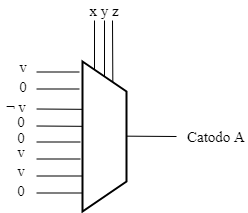
\includegraphics[scale=0.6]{esercizio04/images/MuxA8x1.png}
	\caption{Multiplexer 8x1 che realizza la funzione booleana del segmento A}
	\label{fig:muxA}
\end{figure}

Dopo la costruzione dei vettori degli ingressi per ogni multiplexer,
si � definito un vettore di vettori per consentire una generazione
della struttura mediante il costrutto \emph{for-generate}.

\lstinputlisting[language=VHDL, caption={Architettura Structural del componente Cathode Encoder},firstline=73,lastline=110]{esercizio04/codice/cathode_encoder.vhd}

\paragraph{Dataflow}

Denominati gli ingressi come nel paragrafo precendete, si � provveduto
a definire un file blif per la funzione multi-uscita dei sette segmenti.
In tal modo � stata possibile una minimizzazione con SIS attraverso
l'uso del \emph{rugged-script}.

\begin{figure}[H]
	\centering
	\includegraphics[scale=0.9]{esercizio04/images/7SegRuggedScriptmod.png}
	\caption{Funzione multi-uscita dei sette segmenti minimizzata col rugged-script}
	\label{fig:7segrs}
\end{figure}

Ogni uscita � calcolata in base alla forma minimizzata della funzione
corrispondente.

\lstinputlisting[language=VHDL, caption={Architettura Dataflow del componente Cathode Encoder},firstline=112,lastline=149]{esercizio04/codice/cathode_encoder.vhd}

\subsubsection{Display}

Il display non fa altro che realizzare la struttura descritta in \ref{subsec:display}.
Sono infatti istanziati e collegati nel modo descritto i componenti
cui abbiamo fatto riferimento.

\lstinputlisting [language=VHDL,caption={Definizione del componente Display}] {esercizio04/codice/display.vhd}\selectlanguage{italian}%

